\chapter{Introdução}
\label{ch:intro}

Dentro do ciclo de vida de um produto de software o processo de manutenção tem
papel fundamental. Devido ao seu alto custo, em alguns casos chegando a 60\%
do custo final \cite{kaur2015review}, as atividades relacionadas a manter e evoluir software tem sua
importância considerada tanto pela comunidade científica quanto pela indústria. Neste sentido, este trabalho de dissertação se propõe a investigar e contribuir no entendimento de como as Ferramentas de Gerenciamento de Requisição de Mudança estão sendo melhoradas ou estendidas no contexto da transformação do processo de desenvolvimento e manutenção de software de um modelo tradicional para outro que incorpora cada vez mais as práticas propostas pelos agilistas. O intuito é analisar como as FGRM estão sendo modificadas com base na literatura da área em contraste com o ponto de vista dos profissionais envolvidos em manutenção de software.

A \textit{Manutenção}, dentre outros aspectos, corresponde ao processo de modificar um componente ou sistema de software após a sua entrega com o objetivo de \textit{corrigir falhas, melhorar o desempenho ou adaptá-lo devido à mudanças ambientais} \cite{{159342}}. De maneira relacionada, \textit{Manutenibilidade} é a propriedade de um sistema ou componente de software em relação ao grau de \textit{facilidade} que ele pode ser corrigido, melhorado ou adaptado \cite{{159342}}.

As manutenções em software podem ser divididas em \textit{Corretiva, Adaptativa, Perfectiva e Preventiva} \cite{Lientz:1980:SMM:601062,159342}. A Manutenção Corretiva lida com a reparação de falhas encontradas. A Adaptativa tem o seu foco na adequação do software devido à mudanças ocorridas no ambiente em que ele está inserido. A Perfectiva trabalha para detectar e corrigir falhas latentes antes que elas se manifestem como tal. A  Perfectiva fornece melhorias na documentação, desempenho ou manutenibilidade do sistema. A Preventiva se preocupa com atividades que possibilitem aumento da manutenibilidade do sistema. A \textit{ISO 14764} \cite{1703974} propõe a divisão da tarefa de manutenção nos quatro tipos descritos anteriormente e agrupa-os em um termo único denominado \textit{Requisição de Mudança - Modification Request (RM)}, conforme pode ser visto pela Figura \ref{fig:modification-request}

\begin{figure}[hbtp]
\centering
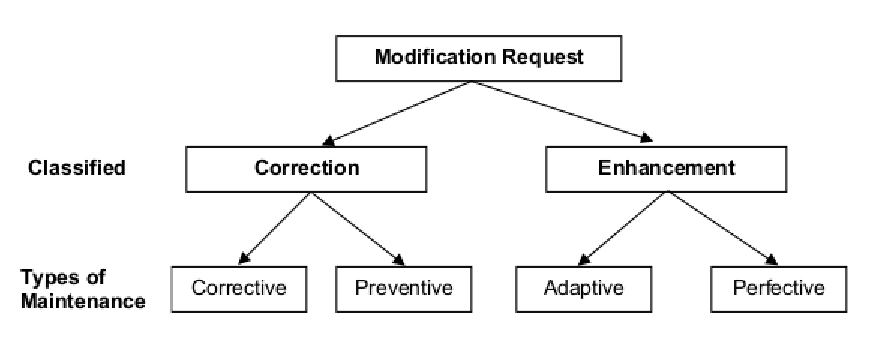
\includegraphics[width=.75\textwidth]{chapter-intro/img/modification_request.eps}
\caption{Tipos de manutenção segundo a norma ISO/IEC 14764. Extraído de
  \cite{1703974}}
\label{fig:modification-request}
\end{figure}

\todo[inline]{Fazer uma discussão melhor sobre as diferenças entre manutenção e evolução de
	Software}
Por conta do volume das Requisições de Mudança se faz necessária a utilização de ferramentas com o
objetivo de gerenciá-las. Esse controle é geralmente realizado por Sistemas de Controle de Demandas
(SCD)- Issue Tracking Systems, que auxiliam os desenvolvedores na correção de forma individual ou
colaborativa de defeitos (bugs), no desenvolvimento de novas funcionalidades, dentre outras tarefas
relativas à manutenção de software. Não existe na literatura uma nomenclatura comum para este tipo
de ferramenta. Em alguns estudos é possível verificar nomes tais como Sistema de Controle de Defeito
- Bug Tracking Systems, Sistema de Gerenciamento da Requisição - Request Management System, Sistemas
de Controle de Demandas (SCD)- Issue Tracking Systems e diversos nomes afins. Todavia, de modo
geral, o termo se refere as ferramentas utilizadas pelas organizações para \textit{gerir as
	Requisições de Mudança}. Estas ferramentas podem ainda ser utilizadas por gestores, analistas de
qualidade e usuários finais para atividades tais como gerenciamento de projetos, comunicação,
discussão e revisões de código. Neste trabalho utilizaremos o termo \texttt{Ferramentas de Gerenciamento de Requisições de Mudança} (FGRM) ao referimos a este tipo de ferramenta.
A Tabela \ref{tab:exemplo} apresenta alguns exemplos de ferramentas que podem ser classificadas como FGRM. Também são listados serviços da Internet que oferecem funcionalidades presentes nas FGRM na forma de Software como Serviço.

\begin{table}[ht]
	\centering
	\resizebox{\textwidth}{!}{%
		\begin{tabular}{llll}
			\hline
			\multicolumn{2}{c}{\textbf{Ferramentas}}           & \multicolumn{2}{c}{\textbf{Serviços da Internet}} \\ \hline
			Bugzilla & https://www.bugzilla.org/               & SourceForge    & https://sourceforge.net/    \\ \hline
			MantisBT & https://www.mantisbt.org/               & Lauchpad       & https://launchpad.net/      \\ \hline
			Trac     & https://trac.edgewall.org/              & Code Plex      & https://www.codeplex.com/   \\ \hline
			Redmine  & www.redmine.org/                        & Google Code    & https://code.google.com/    \\ \hline
			Jira     & https://www.atlassian.com/software/jira & GitHub         & https://github.com/         \\ \hline
		\end{tabular}%
	}
	\caption{Exemplos de ferramentas e serviços da Internet. Adaptado de \cite{cavalcanti2014challenges}}
	\label{tab:exemplo}
\end{table}

Grande parte da literatura de manutenção de software trata de técnicas e metodologias tradicionais da Engenharia de Software. Não obstante, é possível verificar um protagonismo das práticas propostas pelos agilistas em projetos de sucesso, mesmo em áreas não relativas à Tecnologia da Informação \cite{Serrador2015}. Neste contexto, verifica-se uma tendência que os departamentos dedicados à manutenção de software se mostrem interessados nas metodologias dos agilistas e que tenham vontade de experimentá-las em suas atividades \cite{Heeager2015}. Apesar da maioria dos textos em Engenharia de Software tratarem desenvolvimento e manutenção como atividades com natureza distintas, esta última pode adaptar características da primeira visando a melhoria do seu desempenho. Dentre as práticas propostas pelos agilistas passíveis de serem utilizadas em tarefas de manutenção é possível citar o desenvolvimento iterativo, maior envolvimento do cliente, comunicação face a face, testes frequentes, dentre outras.

Da mesma forma que ocorre no desenvolvimento de software, é possível verificar uma crescente adoção
de técnicas da metodologia ágil na manutenção de software \cite{Soltan2016,Devulapally2015,
	Heeager2015}. Neste contexto, é natural que ferramentas que dão suporte à manutenção, tal como
as FGRM's, tenham que evoluir para se adaptar a esta nova forma de trabalhar. Mesmo em um ambiente
tradicional de  desenvolvimento e manutenção de software, verifica-se a necessidade de adequação das
FGRM's. Uma das justificativas desta exigência se deve ao fato que a maioria desses sistemas são
projetados em torno do termo "demanda" (bug, defeito, bilhete, recurso, etc.), contudo, cada vez
mais este modelo parece estar distante das necessidades práticas dos projetos de software,
resultando, por exemplo, que os desenvolvedores tenham um
baixo entendimento da situação geral bem como das atividades das outras pessoas
envolvidas no projeto \cite{Baysal:2013:SAP:2486788.2486957}


Apesar da inegável importância das FGRM's, percebe-se um aparente desacoplamento deste tipo de ferramenta com as necessidades das diversas partes interessadas (stakeholders) na manutenção e evolução de software. Um sinal deste distanciamento pode ser observado pelas diversas extensões (plugins) propostas na literatura \cite{101186,Thung:2014:BIT:2635868.2661678,Kononenko:2014:DED:2591062.2591075}.
 
\section{Justificativa}
\label{sec:intro-justificativa}
Desde o final da década de 1970 \cite{Zelkowitz:1979:PSE:578504} percebe-se o aumento do custo referente as atividades de  manutenção de software. Nas décadas de 1980 e 1990 alguns
trabalhos tiveram seu foco no desenvolvimento de modelos de mensuração do custo
para manter o software \cite{Herrin:1985:SMC:323287.323383,hirota1994approach}. Apesar da evolução das metologias de manutenção a estimativa é que nas últimas duas décadas o custo de manutenção tenha aumentado em 50\% \cite{koskinen2010software}. Esta tendência pode ser observada na Figura \ref{fig:software-maintence-costs} no qual é possível verificar a evolução do custo da manutenção de software como fração do custo total do produto.

\begin{figure}
\centering
\includegraphics[width=0.7\linewidth]{./chapter-intro/img/software-maintence-costs}
\caption{Evolução da manutenção de software como percentual do custo total.	Extraído de	\cite{engelbertink2010save}}

\label{fig:software-maintence-costs}
\end{figure}

Diante da maior presença de software em todos os setores da sociedade
existe um interesse por parte da academia e da industria no desenvolvimento de
processos, técnicas e \textit{ferramentas} que reduzam o esforço e o custo das tarefas
de desenvolvimento e manutenção de software. Neste linha, o trabalho de Yong \& Mookerjee \cite{1423995}  propõe um modelo que reduz os custos de manutenção e reposição durante a vida útil de um sistema de software. O modelo demonstrou que em algumas situações é \textit{melhor substituir um sistema do que mantê-lo}. Este problema é agravado tendo em vista que o custo de manutenção pode chegar a 60\% do custo total do software \cite{kaur2015review}. Este percentual reflete a fração de desenvolvedores dedicados à tarefas de manutenção de sistemas \cite{Zhang_2003}.

A manutenção não necessariamente exige que o processo de software envolvido
seja o tradicional. Percebe-se alguns exemplos de adoção das práticas ágeis
para fins de manutenção e evolução do software \cite{kajko2009model, Heeager2015, Devulapally2015,Naz2016}. Tal
tendência não é surpreendente tendo em vista que os métodos ``ágeis'' enfatizam
características úteis à eficiência da implementação de software, tais como desenvolvimento incremental e teste contínuo que agregam valor para a evolução e manutenção eficaz de um sistema
\cite{thomas2006agile}. Dentro desta tendência verifica-se a necessidade de que as ferramentas envolvidas no suporte à manutenção de software se adequem à este nova forma de manter software. 

O desenvolvimento e a manutenção de software envolvem diversos tipos de métodos,
técnicas e ferramentas. Em especial no processo de manutenção, um importante aspecto são as diversas Requisições de Mudanças que devem ser gerenciadas. Este controle é realizado pelas Ferramentas de Gerenciamento de Requisição de Mudanças (FGRM) cujo o uso vem crescendo em importância, sobretudo, por sua utilização por gestores, analistas da qualidade e usuários finais para atividades como tomada de decisão e comunicação.

A utilização de  \textit{``demanda''} como conceito central para Ferramentas de Gerenciamento de Requisição de Mudanças (FGRM) parece ser distante das necessidades práticas dos projetos de software, especialmente no ponto de vista dos desenvolvedores \cite{Baysal:2013:SAP:2486788.2486957}. Um exemplo deste desacoplamento das FGRM com a necessidade de seus usuários pode ser visto no trabalho proposto por Baysal \& Holme \cite{baysal2012qualitative} no qual desenvolvedores que utilizam o Bugzilla\footnote{\url{https://www.bugzilla.org}} relatam a
dificuldade em manter uma compreensão global das RM's em que eles estão
envolvidos. Segundo os desenvolvedores seria interessante que a ferramenta
tivesse um suporte melhorado para a Consciência Situacional - Situational
Awareness. Em síntese, eles gostariam de estar cientes da situação global do
projeto bem como das atividades que outras pessoas estão realizando. Um outro
sinal da necessidade de evolução deste tipo de ferramenta pode ser observado considerando as diversas extensões (plugins) propostas na literatura \cite{101186,Thung:2014:BIT:2635868.2661678,Kononenko:2014:DED:2591062.2591075}.

Neste contexto, é proposto neste projeto de dissertação a elaboração de um estudo das Ferramentas de Gerenciamento de Requisição de Mudança (FGRM) como o objetivo de \textit{(i)} entender os requisitos comuns deste tipo de ferramenta; \textit{(ii)} mapear as extensões para as FGRM que estão sendo propostas na literatura; \textit{(iii)} avaliar sobre o ponto de vista dos profissionais a situação atual dos FGRM; \textit{(iv)} propor novas extensões para as FGRM. Vamos discutir os aspectos que são
considerados mais importantes a partir da literatura da área bem como do ponto de vista de profissionais envolvidos em manutenção de software. De forma particular, iremos estudar os mecanismos de personalização que algumas destas ferramentas permitem e tentaremos ainda criar exemplos de personalização para alguma possível extensão a ser identificada ao longo do trabalho.

\section{Motivação}
\label{sec:intro-motivacao}

\section{Problema}
\label{sec:intro-problema}

\section{Visão Geral da Proposta}
\label{sec:intro-visao-geral}

\section{Metodologia de Pesquisa}
\label{sec:intro-metodologia}

O trabalho de dissertação pode ser dividido nas etapas listadas a seguir:

\begin{itemize}[(i)]
	\item Mapeamento Sistemático da Literatura \cite{keele2007guidelines}
	\item Caracterização das Ferramentas de Gerenciamento de Requisição de Mudança (FGRM)
	\item Pesquisa (Survey) com os desenvolvedores \cite{wohlin2012experimentation}
	\item Desenvolvimento de extensões para as FGRM's
\end{itemize}

\section{Contribuições da Dissertação}
\label{sec:intro-contribuicao}

\section{Organização da Dissertação}
\label{sec:intro-organizacao-dissertacao}
